\documentclass{article}
    % General document formatting
    \usepackage[margin=0.7in]{geometry}
    \usepackage[parfill]{parskip}
    \usepackage[utf8]{inputenc}
    \usepackage{graphicx}
    \usepackage[sort&compress,numbers,super]{natbib}
    \usepackage{booktabs}
    
    % Related to math
    \usepackage{amsmath,amssymb,amsfonts,amsthm}
    \graphicspath{{figures/}}
\begin{document}
\chapter{Predicting Near Edge X-ray Absorption Spectra with the Spin-Free Exact-Two-Component Hamiltonian and Orthogonality Constrained Density Functional Theory}
\epigraph{\textit{``There is one topic I was NOT sorry to skip: the relativistic wave equation of Dirac''}}{Steven Weinberg}
\begin{chapabstract}
Orthogonality constrained density functional theory (OCDFT) provides near edge X-ray absorption (NEXAS) spectra of first row elements within one electron volt from experimental values.
However, with increasing atomic number, scalar relativistic effects become the dominant source of error in a nonrelativistic OCDFT treatment of core-valence excitations.
In this work we report a novel implementation of the spin-free exact-two-component (X2C) one-electron treatment of scalar relativistic effects, and its combination with a recently developed OCDFT approach to compute a manifold of core-valence excited states.
The inclusion of scalar relativistic effects in OCDFT reduces the mean absolute error of second-row elements core-valence excitations from 10.3 to 2.3 eV.
For all the excitations considered, the results from X2C calculations are also found to be in excellent agreement with those from low-order spin-free Douglas--Kroll--Hess relativistic Hamiltonians.
The X2C-OCDFT NEXAS spectra of three organotitanium complexes (TiCl$_4$, TiCpCl$_3$, TiCp$_2$Cl$_2$) are in very good agreement with \textit{unshifted} experimental results, and show a maximum absolute error of 5--6 eV.
In addition, a decomposition of the total transition dipole moment into partial atomic contributions is proposed and applied to analize the nature of the Ti pre-edge transitions in the three organotitanium complexes.
\end{chapabstract}
\section{Introduction}
The emergence of high-intensity and tunable synchrotron radiation sources has made X-ray absorption techniques some of the most powerful and versatile spectroscopic tools for elucidating local chemical information. Near-Edge X-ray Absorption Spectroscopy (NEXAS) probes electronic transitions from core to unoccupied states below the continuum,\cite{stohr_nexafs} providing a mean to investigate various electronic structure properties of the absorbing atom, such as oxidation state, coordination number, and spin/state symmetry.\cite{Use-NEXAS,NEXAF-use-covant,NEXAFS-oxidation,C2CY00343K}. NEXAS has been applied to a wide range of chemical systems, including: small molecules in the gas phase\cite{small-molecule}, molecules in liquid environments,\cite{Wernet2004,Freiwald2004} large biological systems\cite{Hans-DNA}, thin-films\cite{review-XAS}, and semi-conducting materials\cite{Semi-conductor}. Experimental NEXAS studies are often coupled with computational simulations in order to quantify more subtle electronic structure information like discrete contributions to peak features, covalency, and orbital mixing. \cite{Milne-review,stohr_nexafs,C2CY00343K,NEXAF-use-covant,B926499J}

Computing NEXAS spectra can be challenging since relativistic, relaxation, and correlation effects play a vital role in determining the accuracy of core-excitation energies. Several attempts have been made to extend many-body methods like coupled cluster theory\cite{LR-CC-core,Bartlett-EOM-core,Besley-EOM-MOM,Li-EOM,MRCC-core1, MRCC-core2, MRCC-core3}, configuration interaction\cite{CI_core,CI_core1,Nesse-CI,Asmuruf2008267,Grimme1996128}, and Green's-function approaches\cite{ADC2,Bethe-Salpeter} to compute NEXAS spectra.
NEXAS spectra can also be simulated using computationally less expensive methods such as multiple scattering theory\cite{Rehr-MS,MS-another,PhysRevB.63.125120}, Slater transition state\cite{sTOM}, transition potential\cite{TPT,PhysRevLett.96.215502}, static exchange method\cite{STEX}, configuration interaction singles\cite{SAC-CIS, SAC-CIS-2}, $\Delta \text{SCF}$\cite{Delta-SCF}, linear response time-dependent density functional theory (TD-DFT)\cite{TD-DFT-core,Besley-tddft, TD-DFT-Li}, and real-time TD-DFT\cite{RT-DFT-nwchem,Lopata-recent}.

Due to their low computational cost and ability to treat multiple excited states, methods based on TD-DFT are widely used to compute NEXAS. The accuracy of excitation energies computed with TD-DFT are strongly dependent on the choice of exchange-correlation (xc) kernel. Its failures are often attributed to errors in the Kohn$-$Sham eigenvalues, lack of frequency dependence in  the xc-kernel, and the adiabatic approximation\cite{Casida-review-2012}. For core excitations, TD-DFT provides only reliable relative energies\cite{Besley-Gill} and empirical energy shifts must be used to achieve accurate absolute excitation energies.

Errors associated with the xc kernel and the Kohn$-$Sham orbital energies\cite{DFT_PV_3,DFT_PV_4} can be reduced by using time-independent DFT methods\cite{Besley-Gill,Voorhis,Ziegler-1}. 
We have recently proposed orthogonality constrained DFT (OCDFT),\cite{OCDFT} a variational time-independent approach to compute excited states.
OCDFT builds excited states via a generalized Kohn--Sham (KS) formalism that enforces additional orthogonality constraints between the ground and excited state wave functions.
Our preliminary study\cite{Wallace-OCDFT} on a test set of 40 core-excited states showed that OCDFT produces absolute excitation energies that are more accurate than TDDFT.
For example, using the popular B3LYP functional and a quadruple-$\zeta$ basis set, the mean absolute error for OCDFT and TDDFT is 1.0 and 21.6 eV, respectively. 
Our study found that the performance of nonrelativistic OCDFT was excellent for first-row elements.
However, for second-row elements, relativistic effects were found to be the dominant source of error, and undoubtedly become more important when considering heavier elements. In this study we investigate the issue of relativistic effects in the prediction of K-edge spectra and propose an inexpensive and accurate approach that combines scalar relativistic Hamiltonians with OCDFT.


Since a many-electron relativistic Hamiltonian cannot be easily derived from quantum electrodynamics, the theoretical treatment relativistic effects in electronic structure calculations is still an open problem.\cite{Dyall-book,Wolf-book,moss-book,grant-book,Kutzelnigg2012-review}
The simplest strategy is to decompose the  relativistic effects into different contributions,
i.e., scalar relativistic effects, spin-orbit coupling, magnetic induction, retardation effects, and finite nuclei, and include only those components relevant to the system and property under consideration\cite{Cremer,Reiher-X2C,Rel-review-UB,Rel-review-Trond,Rel-review-Wenjian}. For K-edge X-ray absorption spectroscopy, scalar relativistic effects due to 1s orbital contraction are the dominant contribution, while other effects (e.g. spin-orbit coupling) become dominant when considering transitions from p and d orbitals.\cite{schwerdtfeger-book2,C-imp,Rel-review-UB,Dyall-book}.

A convenient approach to account for scalar relativistic effects consists in using the Foldy--Wouthuysen\cite{FW,Heully} (FW) unitary transformation.
The FW transformation can be used to reduce the four-component Dirac Hamiltonian to an exact or approximate quasi-relativistic 2-component (2C) Hamiltonian.
The FW transformation may also be accompanied by elimination of the spin-dependent (vector) term from the 2C Hamiltonian to give a spin-free (SF) formalism. 
Several approaches that follow this philosophy exist: the zeroth order regular approximation (ZORA)\cite{ZORA-chang,ZORA-VBS,ZORA-VBS-2}, the Douglas--Kroll--Hess method \cite{DKH,DKH-V,DKHn-vW,DKHn-Reiher,DKHn-Hirao}, and various infinite-order schemes, including the normalized elimination of the small component,\cite{Dyall-NESC,X2C-Dyall2001,NESC-X2C,ZFC} the Barysz--Sadlej--Snijde method\cite{BSS-1}, the infinite-order two-component scheme\cite{IOTC-previous,IOTC-eig}, and the exact-2-component approach (X2C).\cite{Kutzelnigg-matrix1, llias, X2C-Liu2006,X2C-KUt-Liu2007,IOTC-trond,X2C-Liu2007,X2C-Liu2009}
These methods differ in the way the FW transformation is performed: ZORA approximates it, the DKH method relies on a perturbative approach, and the infinite-order methods perform an exact transformation (within the computational basis).
Since the ZORA Hamiltonian is not gauge invariant with respect to the energy scale,\cite{ZROA-energy-p-VW,ZORA-fix-energy-scale,Nwchem-zora} it does not yield accurate orbital energies and is therefore unsuitable for computing NEXAS spectra.
The gauge dependency problem can be fixed by using a scaled variant of ZORA\cite{scaled-ZORA,ZORA-fix-energy-scale} or ZORA with a model potential\cite{ZROA-energy-p-VW}. The former is designed to match the Dirac energies of hydrogen-like atoms, while the latter approach uses a model effective nuclear potential in the ZORA operator.
  
In this work we report a new implementation of the spin--free scalar quasi-relativistic X2C Hamiltonian at the one-electron level in the \textsc{psi4} \textit{ab initio} quantum chemistry package\cite{PSI4}. A brief outline of the working equations of X2C is provided along with details of our implementation. We showcase the utility of X2C by characterizing its effect on the computation of OCDFT core excitation energies. The accuracy of NEXAS spectra computed using only scalar relativistic effects will be assessed by evaluating the performance of X2C-OCDFT over a test set of 37 unique core excitations from 13 different molecules spanning the first and second row of the periodic table. The performance of the X2C Hamiltonian will also be compared with that of second-, third-, and fourth-order DKH. The full treatment of relativistic effects enables us to study the NEXAS spectra of second- and third-row elements, which we demonstrate by computing the Ti K-edge of three organotitanium complexes. 

\section{Theory}
\subsection{One-Electron Spin-Free X2C} 
The central idea of the X2C method is to find a transformation that separates the positive (electronic) and negative solutions of the Dirac equation.
More precisely, one seeks a unitary operator $U$ that decouples the positive-energy ($h^{\rm FW}_{++}$) and negative-energy ($h^{\rm FW}_{--}$) blocks of the Dirac Hamiltonian ($h^{\rm D}$):
\begin{equation}
U^\dagger h^{\rm D} U = 
U^\dagger
\begin{pmatrix}
h_{LL} & h_{LS} \\
h_{SL} & h_{SS}
\end{pmatrix}
 U
 =
 \begin{pmatrix}
h^{\rm FW}_{++} & 0 \\
0 & h^{\rm FW}_{--}
\end{pmatrix}
\end{equation}
The transformation $U$ is built from the solutions of the Dirac equation.
The one-electron treatment of X2C neglects the electron-electron interaction, and thus, it is only necessary to solve the one-electron Dirac equation to find $h^{\rm FW}_{++}$.
In a kinetically balanced basis treatment\cite{Kinetic-balance,Dyall-KB} in which the large component is expanded using an atomic orbital basis of dimension $N$, $\{\chi_{\mu}, \mu=1,...,N\}$, the spin-free modified Dirac equation reads:
\begin{equation}
\left(
\begin{array}{cc}
{V}                   &  {T} \\
{T} & \frac{W^{\text{SF}}}{4c^2}-{T} \\ 
\end{array}
\right)
\left(
\begin{array}{c}
{C}^{\text{L}}                   \\
{C}^{\text{S}}  \\ 
\end{array}
\right)  
= \left(
\begin{array}{cc}
{S}                  &  {0}\\
{0} & \frac{{T}}{2c^2} \\ 
\end{array}
\right)
\left(
\begin{array}{c}
{C}^{\text{L}}                    \\
{C}^{\text{S}}  \\ 
\end{array}
\right)  E
\label{eq:Dirac_ham_mine}
\end{equation}
where \textit{c} is the speed of light,  $S$ is the overlap integral, and $T$, $V$, and $W^{\rm SF}$ are the matrix representation of the nonrelativistic kinetic energy ($\hat{p}^2/2$), the nuclear-electron attraction potential ($\hat{V}$), and the spin-free relativistic potential [$\hat{p}\cdot (\hat{V}\hat{p})$], respectively.
The integrals $W^{\rm SF}_{\mu\nu} = \bra{\chi_\mu} \hat{p}\cdot (\hat{V}\hat{p}) \ket{\chi_\nu}$ can be easily computed as derivatives of the nuclear-electron attraction integrals with respect to nuclear coordinates.
Note that the spin-free formulation of X2C simplifies the form of the relativistic potential and leads to a problem that has a lower dimensionality than the full Dirac equation: the matrices that enter the modified Dirac equation  [Eq.~\eqref{eq:Dirac_ham_mine}] have dimension $N \times N$, which leads to a $2N \times 2N$ eigenvalue problem.

In the X2C treatment,\cite{Dyall-NESC,X2C-Dyall2001,Kutzelnigg-matrix1, llias, X2C-Liu2006,X2C-KUt-Liu2007,IOTC-trond,X2C-Liu2007,X2C-Liu2009}  the positive-energy block of the Hamiltonian $h^{\rm FW}_{++}$ is given by the sum of a transformed kinetic ($T_{\text{X2C}}$) and potential energy ($V_{\text{X2C}}$) contribution, defined as
\begin{equation}
	T_{\text{X2C}}= R^{\dagger} (TX +  {X}^{\dagger}T - {X}^{\dagger}TX ) R 
	\label{eq:TQrel}
\end{equation}
and
\begin{equation}
	V_{\text{X2C}} =  R^{\dagger}(V + \frac{1}{4c^2} X^{\dagger}W^{\text{SF}}X) R
	\label{eq:VQrel}
\end{equation}
The coupling matrix ${X} = C^{\text{S}} (C^{\text{L}})^{-1}$ is obtained from the large ($C^{\rm L}$) and small ($C^{\rm S}$) components of the $N$ positive energy solutions of the Dirac equation.
The renormalization matrix\cite{X2C-Liu2009} 
\begin{equation}
{R}=S^{-1/2}(S^{-1/2}\tilde{S}S^{-1/2})^{-1/2}S^{1/2},
\end{equation}
depends on the modified overlap matrix
\begin{equation}
\tilde{S}=S+\frac{1}{2c^2}X^{\dagger}TX.
\end{equation}

Existing nonrelativistic electronic structure code can be extended to include scalar relativistic effects treated with the X2C method by replacing nonrelativistic kinetic and potential energy with the corresponding X2C operators $T_{\text{X2C}}$ and $V_{\text{X2C}}$. 
The X2C one-electron operator is formed before the beginning of the HF/KS-SCF cycle and added to two-electron HF/KS operator. Our X2C implementation in \textsc{psi4} closely follows that reported by Cheng and Gauss\cite{Lan-X2C} in their work on X2C analytic energy gradients.
 
\subsection{Orthogonality Constrained DFT}
Here we will give a brief introduction to orthogonality constrained density functional theory. Extensive details of the OCDFT formalism and its performance to calculate valence-valence excitation energies can be found in ref \citenum{OCDFT}, while details on its extension to treat core excitations and the algorithm used to calculate multiple excited states can be found in ref \citenum{Wallace-OCDFT}.  OCDFT is a variational time independent (TI) formulation of DFT that builds upon the approach developed by Ayers, Levy, and Nagy\cite{ayers_time-independent_2012}, where all $n$ electronic states $\Psi^{(n)}$ of an $N$-electron system have a unique corresponding density functional $E^{(n)}[\rho]$, which is a generalization of the ground state functional $E^{(0)}[\rho]$. The energy functional for state $n$ minimizes the expectation values of the energy while imposing that the trial wave function ($\Psi$) be compatible with the density ($\rho$) and  orthogonal to the first $n$ states: 
\begin{equation}
E^{(n)}[\rho] = \min_{
\substack{
\Psi \rightarrow \rho\\
\Psi\bot \{\Psi^{(k)}\}
}
}
\bra{\Psi}\hat{H}\ket{\Psi}, k = 0,1,...n-1
\end{equation}

OCDFT provides a practical realization of the Ayers--Levy--Nagy TIDFT approach that is based on a generalized Kohn--Sham scheme.
In OCDFT, to each electronic state $\Psi^{(n)}$ corresponds an auxiliary system of noninteracting electrons with wave function $\Phi^{(n)}$ and density $\rho^{(n)}$. 
The wave function for the auxiliary system is a single Slater determinant, $\ket{\Phi^{(n)}} = \ket[1]{\phi_1^{(n)}\phi_2^{(n)} \cdots\phi_N^{(n)}}$, where the set of orbitals $\{\phi_i^{(n)}\}$ are different for each electronic state.
In the derivation of a practical Kohn--Sham scheme for OCDFT, the energy functional is augmented with an orthogonality condition on the auxiliary wave functions
\begin{equation}
\label{eq:OCcondition}
\langle \Phi^{(m)} | \Phi^{(n)} \rangle = \delta_{mn} \;\;\;  \forall m,n
\end{equation}
This orthogonality condition prevents the excited state from optimizing down to the ground state solution, effectively avoiding the variational collapse problems that plague most $\Delta$SCF methods.
In the resulting variational KS method, every excited state has an associated energy functional $E^{(n)}_{\rm KS}[\{\phi^{(n)}_i\}]$ which has a unique exchange-correlation (xc) contribution $E^{(n)}_{\rm xc}$.

\begin{figure*}[h!]
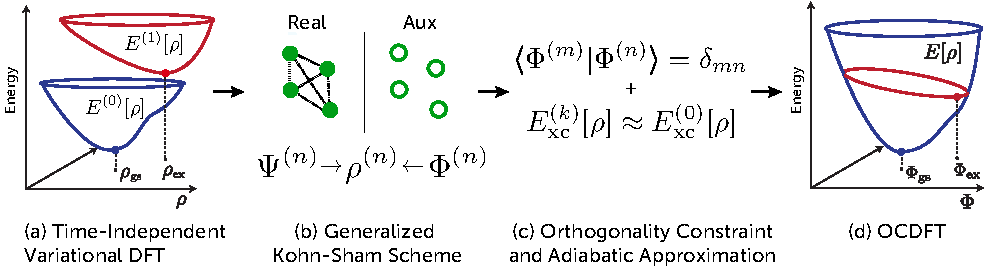
\includegraphics[width=6.5in]{figure_1.pdf}
\caption{Outline of Orthogonality Constrained DFT: (a) In the Ayers--Levy--Nagy time-independent variational formulation of DFT each electronic is associated with a unique density functional. (b) For each electronic state $\Psi^{(n)}$, an auxiliary system of non-interacting electrons with wave function $\Phi^{(n)}$ is introduced.   $\Psi^{(n)}$ and $\Phi^{(n)}$ are assumed to have the same electron density $\rho^{(n)}$. (c) We then impose explicit orthogonality conditions onto the auxiliary wave functions and approximate the unknown exchange-correlation (xc) functional $E_{\rm xc}^{(n)}$ with the ground-state functional. (d) The final OCDFT functional consists in the ground state functional augmented with an orthogonality constraint.}
\label{fig: OCDFTderiv}
\end{figure*}

%Defining a generalized Kohn--Sham system, we introduce 
As illustrated in Figure~\ref{fig: OCDFTderiv}, OCDFT invokes an adiabatic approximation similar to the one adopted in TDDFT, in which the xc contribution for each excited state is approximated by the ground state functional $E^{(0)}_{\rm xc}$. This results in the OCDFT functional for excited state $n$, which is given by:
\begin{equation}
\begin{split}
E^{(n)}_{\rm OCDFT}[\{\phi^{(n)}_i\}] =& - \frac{1}{2} \sum^{\rm occ}_i \langle \phi^{(n)}_i| \nabla^2 |\phi^{(n)}_i \rangle \\
 &+ \int d\textbf{r} \;  v_{\text{ext}}(\textbf{r}) \rho(\textbf{r}) \\
&+  E_{\text{Coul}}[\rho^{(n)}] + E^{(0)}_{\text{xc}}[\rho^{(n)}]
\label{eq:OCDFT_E_ORIGINAL}
\end{split}
\end{equation}
where $v_{\text{ext}}(\textbf{r})$ is the external potential and $E_{\text{Coul}}[\rho^{(n)}]$ is the classical electron-electron interaction energy term.

In this work we solve the OCDFT equations via our constrained multiple hole/particle (CMHP) algorithm.\cite{Wallace-OCDFT}
Within the CMHP scheme, each excited state is characterized by a pair of hole ($\phi_{\rm h}^n$) and particle ($\phi_{\rm p}^n$) orbitals, which are required to span the occupied and virtual space of the ground state wave function, respectively.  These may be interpreted as the orbitals from which an electron is annihilated and created as a result of an electronic excitation.
Rather than solving for the minimum orthogonality conditions between the states, the CMHP algorithm exploits the locality of hole orbitals in core-excited states by imposing sufficient \textit{orbital orthogonality conditions}. This approximation simplifies the Lagrangian, producing a computationally feasible minimization procedure.
In addition, it allows us to readily compute multiple excited states by enforcing mutual orthogonality conditions between the hole and particle orbitals of each subsequent excited state.
At the same time, the CMHP scheme fully accounts for relaxation of the remaining spectator orbitals. 

\subsection{Comparison of OCDFT and TDDFT for Core Excitations}
We have previously shown that OCDFT yields core excitation energies that are in better agreement with experiment than TDDFT.\cite{Wallace-OCDFT}
Specifically, we find that OCDFT excitation energies either do not require shifting, or if an energy shift is necessary, it is significantly smaller than the typical values used in TDDFT.
In this section we address the following questions:
1) Why do TDDFT core-excitation spectra require larger energy shifts than OCDFT?
and, 2) How much do \textit{shifted} TDDFT and OCDFT core-excitation spectra differ?

To showcase the differences between TDDFT and OCDFT, we computed the carbon and oxygen K-edge spectra of CO using a series of functionals with increasing amount of Hartree--Fock exchange.
For comparison, we also include results from time-dependent Hartree--Fock (TDHF) and orthogonality-constrained Hartree--Fock (OCHF).
In this example, we will not consider the effect of relativity since for C and O these contribute to shifts in the excitation energies of the order of 0.1--0.3 eV (see Section~\ref{sec:calibration}).
We will denote the fraction of Hartree--Fock exchange included in a functional with the letter $\delta$, and for simplicity we exclude range-corrected functionals from our analysis.

Figure~\ref{fig: C1s} shows the relative peak positions of the OCDFT and TDDFT spectra and the corresponding energy shift necessary to match the C$_{1\text{s} \rightarrow \pi^*}$ and O$_{1\text{s} \rightarrow \pi^*}$ peaks with their experimental values (287.40 and 534.10 eV for C and O, respectively).  See the supplementary material for a table with the data used to create this figure.
Note that for TDDFT, the C spectrum energy shift ranges from $-$6.96 (TDHF, $\delta = 1$) to +16.24 eV (BLYP, $\delta = 0$), while the O spectrum energy shift spans an even wider range (from $-$15.95 to +21.97 eV).
In comparison, OCDFT shifts are smaller, and range from $+$0.25 eV (OCHF) to +0.99 eV (BLYP) for carbon, and from $+$0.87 eV (BHLYP) to +1.77 eV (OCHF) for oxygen.


Figure~\ref{fig: C1s} also shows the relative position of the second, third, and fourth peaks of the K-edge spectrum.
In TDDFT, the position of these three transitions is heavily dependent on the amount of Hartree--Fock exchange.
In accordance with previous studies,\cite{Besly-57p} we note that only a functional with a large fraction of Hartree--Fock exchange like BHLYP ($\delta = 0.5$) can yield TDDFT relative excitation energies that are in sufficient agreement with experiment.
This does not seem to be the case for OCDFT.  Indeed, OCDFT relative peak positions are mostly insensitive to the choice of the functional being used, and surprisingly, both functionals with no (BLYP) and 100\% (HF) Hartree--Fock exchange yield C and O K-edge spectra that are in good agreement with the experimental spectra.
Overall, this example shows that there are fundamental differences between core excitation energies predicted by TDDFT and OCDFT.
%In addition to differences in the peak positions, there will also be differences in the predicted oscillator strengths.
In addition, there will also be differences in the oscillator strengths predicted by TDDFT and OCDFT. 
\begin{figure*}[h!]
	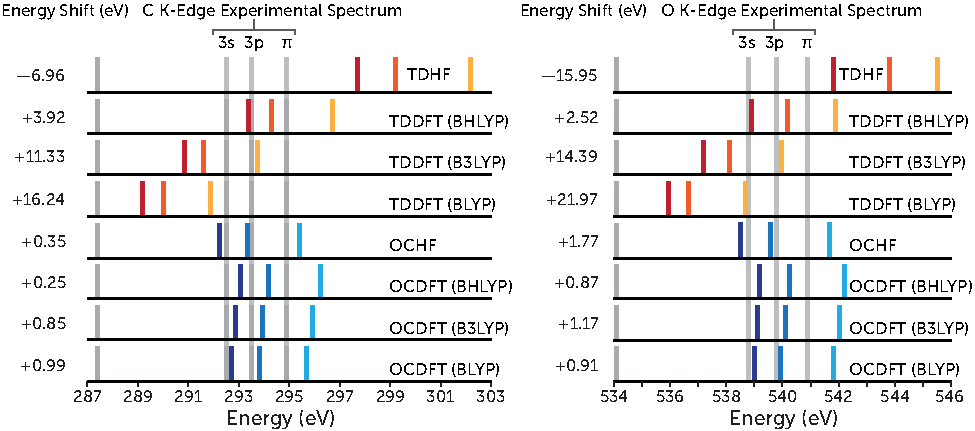
\includegraphics[width=6.5in]{figure_2.pdf}
	\caption{Relative Peak Positions of the C (left) and O (right) K-edge spectra of CO.
	Spectra are shifted by the amount required to align the first peak to the experimental peak values (287.40 and 534.10 eV for the C and O spectrum respectively).  All calculations use the aug-cc-pVQZ basis set.}
	\label{fig: C1s}
\end{figure*}

To understand the differences between TDDFT and OCDFT we analyze a model that captures the essential features of core-excited states.
The model used here is similar to that considered by Casida et al.\cite{Casida-TDDFT-CT-problem} and by Ziegler et al. \cite{Zeigler-TDDFT-CT-problem}.
We consider a system with three orbitals ($\phi_i$ , $\phi_a$, $\phi_b$) of different spatial symmetry.  The ground state of the model is assumed to be the closed-shell determinant $\ket{(\phi_i)^2}$, so that $\phi_a$ and $\phi_b$ are unoccupied orbitals.
We model K-edge transitions as ``charge-transfer-like'' states, that is we assume that the core orbital $\phi_i$ has negligible spatial overlap with virtual orbitals.  This assumption translates in to the condition $\int d\mathbf{r} |\phi_i(\mathbf{r})|^2 |\phi_p(\mathbf{r})|^2 = 0$ for $\phi_p$ equal to $\phi_a$ or $\phi_b$.

We consider the singlet core excitation energies for the transitions $\phi_i \rightarrow \phi_a$ ($\omega_{ai}$) and $\phi_i \rightarrow \phi_b$ ($\omega_{bi}$), together with the relative excitation energy $\Delta \omega = \omega_{bi} - \omega_{ai}$.
For this model, these excitation energies can be written down explicitly in terms of molecular integrals.\cite{Casida-TDDFT-CT-problem,Zeigler-TDDFT-CT-problem}
The reference excitation energies for our model are computed using CIS and are reported in Table \ref{table:OCDFT-CIS-TDDFT}.
In addition, we report the same quantities as obtained from TDDFT using the Tamm--Dancoff approximation and OCDFT with the exchange-correlation functional approximated as a Taylor expansion around the ground state density.
We refer the reader to Table \ref{table:OCDFT-CIS-TDDFT} for the definition of the integrals used in this section.

\begin{table*}[t!]
%	\center
	\caption{Singlet Excitation Energies for a Toy Model of Two Electrons in Three Molecular Orbitals.}
	\begin{tabular}{ll}
		\toprule
Method & Singlet excitation energy$^{a}$ \\
\midrule\\[-8pt]
CIS &   
 $\omega_{ai}^{\rm{CIS}} = h_a - h_i + J_{ai}-J_{ii}$ \\[6pt]
&$ \Delta \omega^{\rm{CIS}}= \omega_{bi} - \omega_{ai} = h_b-h_a  + J_{bi}- J_{ai}$ \\
\midrule
TDDFT 
&$\displaystyle\omega_{ai}^{\rm{TDDFT}} = \omega_{ai}^{\text{CIS}} 
+ (1-\delta) \left(v^{\text{x}}_{a} - v^{\text{x}}_{i} + J_{ai} -  J_{ii} \right)$\\[6pt] 
&$\displaystyle\Delta \omega^{\rm{TDDFT}} = \Delta\omega^{\text{CIS}} + (1-\delta) \left(v^{\text{x}}_{b}
-v^{\text{x}}_{a} + J_{bi} -  J_{ai}\right)$\\  
 \midrule
OCDFT 
& $\displaystyle\omega_{ai}^{\rm{OCDFT}}  = \omega^{\text{CIS}}_{ai} + (1-\delta)\left(v^{\text{x}}_{a}
  -v^{\text{x}}_{i} + \frac{1}{2} J_{aa} - \frac{1}{2} J_{ii}  
  +  \frac{1}{2} f^{\rm x}_{aa} +  \frac{1}{2} f^{\rm x}_{ii} \right)$\\[12pt] 
&$\displaystyle\Delta \omega^{\text{OCDFT}} = \Delta\omega^{\text{CIS}} +
(1-\delta)\left(v^{\text{x}}_{b}
-v^{\text{x}}_{a} + \frac{1}{2}J_{bb} -  \frac{1}{2} J_{aa}
+  \frac{1}{2} f^{\rm x}_{aa}- \frac{1}{2} f^{\rm x}_{bb}\right)$ \\
\bottomrule\\
\multicolumn{2}{l}{
\begin{minipage}{5in}%
\small
{$^a$}The ground state wave function is given by $|\Phi \rangle = | (\phi_i)^2\rangle$. All energies are expressed in terms of one-particle energies, $h_p=\langle\phi_p|\hat{h}|\phi_p\rangle$, density functional exchange potential $v^{\text x}_p = \langle \phi_p|v_{\text{x}}|\phi_p\rangle$, Coulomb $J_{pq}=(pp|r_{12}^{-1}|qq)$, and exchange kernel $f^{\rm x}_{pp} = (pp|f^{\alpha\alpha}_x|pp)$ integrals. The excitation energy of OCDFT is computed by a second-order expansion of the exchange-correlation functional around the ground state density. All contributions arising  from the correlation functional were neglected and minimum overlap between involved orbital is assumed $(\langle|\phi_a|^2 ||\phi_i|^2\rangle\sim 0 )$. The amount of Hartree--Fock exchange included in the density functional is indicated with $\delta \in [0,1]$.
\end{minipage}%
}
\end{tabular} \\

	\label{table:OCDFT-CIS-TDDFT}
\end{table*}

The origin of the large energy shift required to match TDDFT K-edge spectra with experiment may be traced down to the difference between the TDDFT and CIS excitation energy:
\begin{equation} \label{eq:tddft_error}
\omega_{ai}^{\rm{TDDFT}} - \omega_{ai}^{\text{CIS}} = (1-\delta) \left(v^{\text{x}}_{a} -v^{\text{x}}_{i} + J_{ai} -  J_{ii}\right).
\end{equation}
In the local density approximation (LDA), the exchange potential is equal to $v^{\rm x}[\rho] = - \frac{4}{3} C_x \rho^{1/3}$, where $C_x$ is a positive constant.
Therefore, we estimate that the matrix element $v^{\rm x}_{p} = \langle \phi_p|v_{\text{x}}|\phi_p\rangle$ will be larger for orbitals localized near regions with high electron density (i.e. atomic nuclei).  
As a consequence, for core excitations the term $v^{\rm x}_{a} -v^{\rm x}_{i}$ will be positive.
Indeed, for the lowest K-edge transition of CO we estimate this quantity from the full exchange-correlation potential as $v^{\rm xc}_{a} -v^{\rm xc}_{i}$, and find that it is about +48.4 eV for C and +70.9 eV for O.

Let us now turn to the contribution from the second term in Eq~\eqref{eq:tddft_error}, $J_{ai} -  J_{ii}$.
This term can be interpreted physically as the sum of the energy released from breaking the core electron pair ($-J_{ii}$) and the interaction of the unpaired electrons in the hole and particle orbitals ($J_{ai}$).
This term is already present with the correct prefactor in the CIS expression for the excitation energy ($\omega_{ai}^{\rm{CIS}}$), therefore, in the case of TDDFT it is double counted.
For core excitations one has that $J_{ii} \gg J_{ai}$.  Therefore, the second term in Eq~\eqref{eq:tddft_error} is negative, and has the net effect of shifting down the excitation energies.
Since TDDFT core excitation energies are always underestimated, we expect that $J_{ai} -  J_{ii}$ is larger in magnitude than the term $v^{\rm x}_{a} -v^{\rm x}_{i}$.
Indeed, in the case of the lowest energy transition, we find that $J_{ai} -  J_{ii}$ is respectively $-89.7$ and $-123.4$ eV for the C and O K-edge.
Combining these estimates with those for the exchange contributions, we predict TDDFT energy shifts of the order of $-41.4$ eV for C and $-52.1$ eV for O.
These estimates do not agree well with the TDDFT actual shifts, but they still capture some of the essential features of our data for CO: 1) they predict negative shifts that are dominate by the two-electron repulsion contribution, and 2) they predict that the oxygen energy shift is larger in magnitude than that required for carbon.
Note that this model predicts that as the percentage of Hartree--Fock exchange is increased ($\delta \rightarrow 1$), the TDDFT core excitation energies require less shifting.
This observation is in agreement with numerical results.
Indeed, one way to improve the accuracy of TDDFT for core excitation energies is to use functionals with a relatively high fraction of Hartree--Fock exchange (50--60\%).\cite{Besly-57p}

In the case of OCDFT, the equation for the energy shift differs from that of TDDFT and it is somewhat more difficult to analyze.
In addition to a term proportional to $v^{\rm x}_{a} -v^{\rm x}_{i}$, which is also common to the TDDFT expression, the OCDFT shift has various contributions from several local self-interaction terms.
Focusing on the contribution from the two-electron interactions, $\frac{1}{2}(J_{aa} - J_{ii})$, this quantity is equal to $-61.9$ and $-45.0$ eV for O and C, respectively.
In comparison to the TDDFT two-electron contribution, the magnitude of this term is smaller and there is better cancellation of errors.

Turning to our second question, we use the three-state model to compute the relative excitation energies for both the TDDFT and OCDFT spectra.
The excitation energy difference  between the two single excitations as predicted by TDDFT ($\Delta \omega^{\rm{TDDFT}} = \omega_{bi}^{\rm{TDDFT}} - \omega_{ai}^{\rm{TDDFT}}$) differs from the CIS value by the quantity $(1-\delta) \left(v^{\text{x}}_{b}-v^{\text{x}}_{a} + J_{bi} -  J_{ai}\right)$.
The most worrisome contribution to the error is the difference $J_{bi} -  J_{ai}$, which effectively introduces a distance dependence in the excitation energy error.

In the case of OCDFT, the relative excitation energy differs from the CIS value by a combination of exchange potential integrals ($v_b^x - v_a^x$, which also contributes to the TDDFT error) and a sum of differences of self-interaction energies for orbitals $\phi_a$ and $\phi_b$.
Thus, all the terms that contribute to the OCDFT relative energy error are local, and relative excitation energies should not show a marked dependence on the distance between the hole and particle orbitals.

\section{Computational Details}
Core excitation energies are computed with OCDFT using the nonrelativistic Hamiltonian, the spin-free X2C Hamiltonian, and the second-, third-, and fourth-order variants of the DKH (DKH2--4) Hamiltonian. Benchmark core excitation energies were computed for 13 small molecules (CH$_4$, C$_2$H$_4$, HCN, CO, H$_2$CO, N$_2$, N$_2$O,
 SO$_2$, SiH$_4$, PH$_3$, H$_2$S, HCl, Cl$_2$).
The geometries of the test set molecules were optimized with nonrelativistic DFT using Becke's B3LYP \cite{becke_new_1993,lee_development_1988,vosko_accurate_1980,stephens_ab_1994} exchange-correlation functional and the def2-QZVP \cite{weigend_balanced_2005,weigend_accurate_2006} basis set. Individual excitation energies are compared with data obtained from gas-phase NEXAS experiments\cite{puttner_vibrationally_1999,remmers_high-resolution_1992,CO-expt-Kedge,chen_k-shell_1989,tronc_nitrogen_1980,tronc_carbon_1979,francis_studies_1994,adachi_vibronic_1999,hitchcock_k-shell_1979,domke_carbon_1990,nayandin_angle-resolved_2001,bodeur_single-and_1990,gedat_s_1998,hudson_high-resolution_1994,cavell_chemical_1999,bodeur_photoabsorption_1985}.

Geometries for the three titanium complexes used in the study are taken from ref.\citenum{TiCl4} and \citenum{TiCl4-Zeigler}.  The first is a simple tetrahedral TiCl$_4$ complex, while the other two are the mono- and bis-cyclopentadienyl (Cp) complexes TiCpCl$_3$ and TiCp$_2$Cl$_2$. The geometries used in our computations show only small deviations from crystal structures (changes of less than 0.02 $\AA$ in bond length and 0.5$^{\circ}$ in bond angle). OCDFT results for titanium complexes are obtained with the fully uncontracted cc-pVDZ\cite{cc-pvdz-dk-Al-Ar,cc-pvdz-dk-H-Ne} (un-cc-pVDZ) basis set with the two-electron integrals approximated using a density fitting approximation\cite{DF-def2-TZVP-JK,DF-def2-TZVP-JK-1,BAERENDS197341,B000027M,DF-SABIN} with the def2-TZVP-JK auxiliary basis\cite{JCC20702}. For the test set, the fully uncontracted  aug-cc-pVDZ\cite{aug-cc-pvdz-B-F}  (un-aug-cc-pVDZ) basis set was used without the density fitting approximation.
Fully uncontracted basis sets are required to provide a proper description of the small component of the wave function and to guarantee a fair comparison between nonrelativistic and relativistic methods. For these organotitanium complexes, OCDFT core excitation energies are computed using only the X2C Hamiltonian.

 X2C-OCDFT calculations are performed with the \textsc{psi4} \textit{ab initio} quantum chemistry package\cite{PSI4} using our implementation of X2C in \textsc{psi4}.  DKH+OCDFT calculations are performed with \textsc{psi4} using the code of Reiher, Wolf, and Hess\cite{DKHn-Reiher,DKH}. All TD-DFT calculatons are done with the ORCA software package version 3.0.3\cite{ORCA}. Natural population analysis on the Ti complexes were performed using the \textsc{janpa}\cite{nikolaienko_janpa:_2014} software package.

\section{Results and Discussion}
\label{sec:calibration}
\subsection{Calibration of X2C-OCDFT Core Excitation Energies}
In order to gauge the importance of relativistic effects in OCDFT core excitation energies, nonrelativistic (NR) and relativistic computations are performed on a test set of 36 transitions from 13 molecules containing first- and second-row elements. 

\begin{table*}[t!]
\center
\caption{Excitation energies of the three lowest energy 1s core excitations for each atom in CO calculated with X2C-OCDFT using the B3LYP functional and fully uncontracted cc-pV$X$Z and aug-cc-pV$X$Z basis sets ($X$ = D, T, Q). Experimental values are taken from Refs. \citenum{CO-expt-Kedge} and \citenum{tronc_carbon_1979}. Errors greater than 1 eV are indicated with bold font.}
\begin{tabular}{ccrrrrrr}
\toprule
Transition & Exp. & \multicolumn{3}{c}{un-cc-pV$X$Z}& \multicolumn{3}{c}{un-aug-cc-pV$X$Z} \\ \cmidrule(r){3-5}  \cmidrule(l){6-8}
 & & D \space & T \space & Q \space & D \space & T \space & Q \space \\
\midrule
O$_{1\mathrm{s} \rightarrow \pi^*}$ & 534.1 & $-$0.4 & $-$0.8 & $-$0.9 & $-$0.4 & $-$0.8 & $-$0.9 \\
O$_{1\mathrm{s} \rightarrow 3\mathrm{s}}$ & 538.8 & \textbf{3.9} & \textbf{1.9} & 0.9 & 0.0 & $-$0.5 & $-$0.6 \\
O$_{1\mathrm{s} \rightarrow 3\mathrm{p}}$ & 539.8 & \textbf{7.8} & \textbf{4.1} & \textbf{2.4} & 0.1 & $-$0.5 & $-$0.6 \\
C$_{1\mathrm{s} \rightarrow \pi^*}$ & 287.4 & $-$0.5 & $-$0.8 & $-$0.8 & $-$0.5 & $-$0.8 & $-$0.9 \\
C$_{1\mathrm{s} \rightarrow 3\mathrm{s}}$ & 292.5 & \textbf{4.0} & \textbf{2.1} & \textbf{1.1} & 0.0 & $-$0.4 & $-$0.5 \\
C$_{1\mathrm{s} \rightarrow 3\mathrm{p}}$ & 293.4 & \textbf{7.1} & \textbf{4.0} & \textbf{2.4} & 0.3 & $-$0.2 & $-$0.3 \\[3pt]
MAE & & \textbf{4.0} & \textbf{2.3} & \textbf{1.4} & 0.2 & 0.5 & 0.6 \\ 
\bottomrule
\end{tabular}
\label{table:Basis}
\end{table*}

Table \ref{table:Basis} shows the systematic convergence of X2C-OCDFT on a test case of six core excitations of CO using the fully uncontracted correlation consistent cc-pV$X$Z and aug-cc-pV$X$Z series of basis sets ranging from double- to quadruple-$\zeta$ quality. Both 1s $\rightarrow$ $\pi^*$ excitations in CO are represented well across all the basis sets considered, with the addition of diffuse functions having no significant impact on the accuracy of the excitation energies compared to experiment. However, the cc-pV$X$Z series of basis sets struggle to properly describe the 1s $\rightarrow$ 3s and 1s $\rightarrow$ 3p transitions in CO, and the inclusion of diffuse functions drastically improves the accuracy of these excitation energies.
The un-aug-cc-pVDZ basis set provides a convenient compromise between accuracy and cost, and was chosen to benchmark the full test set of core excitations.

 \begin{figure}[!t]
 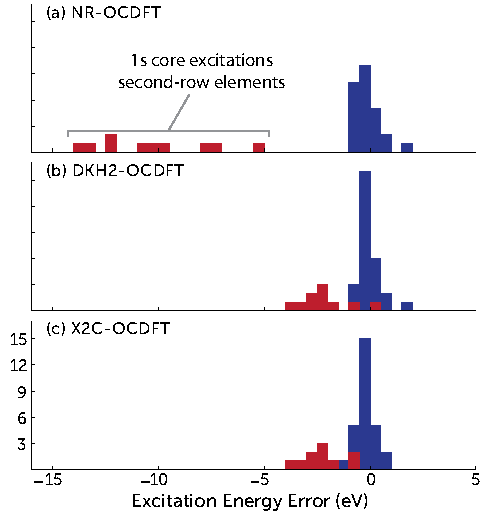
\includegraphics{figure_3.pdf}
 \caption{Error distribution in the computed core excited states for: (a) nonrelativistic OCDFT, (b) OCDFT with the second-order Douglas--Kroll--Hess Hamiltonian, and (c) OCDFT with the exact-2-component Hamiltonian. All calculations use the B3LYP functional and a fully uncontracted aug-cc-pVDZ basis set.  Red bars indicate core excitations from 1s orbitals of second-row elements.}
 \label{fig:histogram}
 \end{figure}

Table \ref{table:FirstRow} and \ref{table:SecondRow} report core excitations from first- and second-row elements.
The performance of OCDFT for \textit{first-row} core excitations is slightly improved upon inclusion of scalar relativistic effects.
Going from NR-OCDFT to OCDFT with scalar relativistic Hamiltonians (X2C, DKH2--4) reduces the error by about 0.2 eV.
In addition, the maximum absolute deviation between X2C-OCDFT and NR-OCDFT for first-row core excitations is only 0.4 eV (O$_{\text{1s}\rightarrow\text{3s}}$ transition of N$_2$O).
X2C and low-order DKH methods yield results that are identical, with negligible differences in MAE.
This similarity in performance between NR-OCDFT and multiple scalar relativistic Hamiltonians is consistent with the general observation that scalar relativistic effects are not significant for the core excitation energies of first row elements.\cite{Asmuruf2008267,Wallace-OCDFT,Besley-EOM-MOM}  A similar conclusion can be drawn from the second row 2$\text{p}$ excitation energies shown in the bottom half of Table \ref{table:SecondRow} where the difference in MAE between NR and relativistic OCDFT is negligible, with identical results produced across all orders of DKH. 

\begin{table*}[t!]
	\caption{OCDFT core excitation energies for molecules containing first-row elements using nonrelativistic (NR) and relativistic (X2C,DKH2, DKH3, DKH4) Hamiltonians. Computations were performed using the uncontracted aug-cc-pVDZ basis with the B3LYP exchange-correlation functional ($E^{\text{B3LYP}}_{\rm xc}$) and 100\% non-local exact exchange ($E^{\text{HF}}_{\rm x}$). OCDFT results are reported here as deviations from the experimental excitation energies (in eV).  The mean absolute error (MAE) is also reported for each method. Experimental values are taken from refs \citenum{puttner_vibrationally_1999,remmers_high-resolution_1992,CO-expt-Kedge,chen_k-shell_1989,tronc_nitrogen_1980,tronc_carbon_1979,francis_studies_1994,adachi_vibronic_1999,hitchcock_k-shell_1979,domke_carbon_1990}.}
\begin{tabular}{lllrrrrrr}
\toprule
Molecule & Excitation   & Exp.  & \multicolumn{6}{c}{Error} \\  \cmidrule(l){4-9}
&            &           &   \multicolumn{5}{c}{$E^{\text{B3LYP}}_{\rm xc}$} & $E^{\text{HF}}_{\rm x}$ \\ \cmidrule(l){4-8} 
&            &           &   NR &  ${\text{X2C}}$ & ${\text{DKH2}}$ & ${\text{DKH3}}$ & ${\text{DKH4}}$ & X2C \\
\midrule
CO 	 		& C$_{\text{1s}\rightarrow\pi^*}$ & 287.4 & $-$0.6 & $-$0.6 & $-$0.5 & $-$0.5 & $-$0.5 & 0.1 \\
			 & C$_{\text{1s}\rightarrow\text{3s}}$ & 292.4 & 0.0 & 0.0 & 0.1 & 0.1 & 0.1 & 0.0 \\
			 & O$_{\text{1s}\rightarrow\pi^*}$ & 534.2 & $-$0.9 & $-$0.5 & $-$0.5 & $-$0.5 & $-$0.5 & $-$1.1 \\
			 & O$_{\text{1s}\rightarrow\text{3s}}$ & 538.9 & $-$0.5 & $-$0.5 & $-$0.1 & $-$0.1 & $-$0.1 & $-$1.2 \\
H$_2$CO 	&  O$_{\text{1s}\rightarrow\pi^*}$ & 530.8 & $-$0.6 & $-$0.2 & $-$0.2 & $-$0.2 & $-$0.2 & $-$0.8 \\
		 & O$_{\text{1s}\rightarrow\text{3s}}$ & 535.4 & $-$0.5 & $-$0.2 & $-$0.2 & $-$0.2 & $-$0.2 & $-$1.3 \\
		& C$_{\text{1s}\rightarrow\text{3s}}$ & 290.2 & $-$0.3 & $-$0.2 & $-$0.2 & $-$0.2 & $-$0.2 & $-$0.6 \\
		 & C$_{\text{1s}\rightarrow\pi^*}$ & 286.0 & $-$0.4 & $-$0.3 & $-$0.3 & $-$0.3 & $-$0.3 & $-$0.2 \\
N$_2$O & O$_{\text{1s}\rightarrow\pi^*}$ & 534.8 & $-$0.5 & $-$0.2 & $-$0.1 & $-$0.1 & $-$0.1 & $-$1.3 \\
		 & O$_{\text{1s}\rightarrow\text{3s}}$ & 536.7 & $-$0.6 & $-$0.2 & $-$0.2 & $-$0.2 & $-$0.2 & $-$3.1 \\
		 & $^c$N$_{\text{1s}\rightarrow\text{3s}}$$^{a}$ & 407.5 & 0.2 & 0.3 & 0.3 & 0.3 & 0.3 & 39.2$^{b}$ \\
		 & $^t$N$_{\text{1s}\rightarrow\pi^*}$$^{a}$ & 401.1 & $-$0.8 & $-$0.5 & $-$0.6 & $-$0.6 & $-$0.6 & 10.4$^{b}$ \\
N$_2$	 & N$_{\text{1s}\rightarrow\pi^*}$ & 401.0 & $-$0.8 & $-$0.5 & $-$0.5 & $-$0.5 & $-$0.5 & 8.9$^{b}$ \\
HCN 	& C$_{\text{1s}\rightarrow\pi^*}$ & 286.4 & $-$0.3 & $-$0.2 & $-$0.2 & $-$0.2 & $-$0.2 & $-$0.3 \\
		 & C$_{\text{1s}\rightarrow\text{3s}}$ & 289.1 & $-$0.2 & $-$0.1 & $-$0.1 & $-$0.1 & $-$0.1 & $-$0.4 \\
		 & N$_{\text{1s}\rightarrow\pi^*}$ & 399.7 & $-$0.6 & $-$0.4 & $-$0.4 & $-$0.4 & $-$0.4 & $-$0.6 \\
		 & N$_{\text{1s}\rightarrow\text{3s}}$ & 401.8 & 0.2 & 0.4 & 0.4 & 0.4 & 0.4 & $-$1.0 \\
CH$_4$	   & C$_{\text{1s}\rightarrow\text{3p}}$ & 288.0 & $-$0.3 & $-$0.2 & $-$0.2 & $-$0.2 & $-$0.2 & $-$0.3 \\
           & C$_{\text{1s}\rightarrow\text{3s}}$ & 287.1 & $-$0.7 & $-$0.6 & $-$0.6 & $-$0.6 & $-$0.6 & $-$0.6 \\
C$_2$H$_2$ & C$_{\text{1s}\rightarrow\pi^*}$ & 285.8 & $-$0.5 & $-$0.3 & $-$0.4 & $-$0.4 & $-$0.4 & 7.6$^{b}$ \\[3pt]
MAE       & &  & 0.5  & 0.3 & 0.3 & 0.3 & 0.3 & 0.8 \\	
\bottomrule		
	\end{tabular}\\	
	$^{a}$The subscripts c and t stand for the center and tail nitrogen of N$_2$O, respectively.\\
	$^{b}$Excitation excluded from the computation of the MAE.
	\label{table:FirstRow}
\end{table*}

Figure \ref{fig:histogram} shows the distribution of errors for all the test set transitions computed with the NR, X2C, and DKH2 Hamiltonians.
Note how the 1s orbital (K-edge) transitions for second-row elements (shaded red in Figure \ref{fig:histogram}) are consistently underestimated by NR-OCDFT and yield a MAE of 10.3 eV.
These troublesome transitions are drastically improved with the inclusion of scalar relativistic effects, reducing the MAE down to 2.3 eV.
Even for excitations that involve second-row element we notice that the X2C and DKH2--4 methods are in excellent agreement (difference in energy less than 0.1 eV).

\begin{table*}[t!]
	\caption{OCDFT core excitation energies for molecules containing first-row elements using nonrelativistic (NR) and relativistic (X2C,DKH2, DKH3, DKH4) Hamiltonians. Computations were performed using the uncontracted aug-cc-pVDZ basis with the B3LYP exchange-correlation functional ($E^{\text{B3LYP}}_{\rm xc}$) and 100\% non-local exact exchange ($E^{\text{HF}}_{\rm x}$). OCDFT results are reported here as deviations from the experimental excitation energies (in eV).  The mean absolute error (MAE) is also reported for each method.
Experimental values are from refs \citenum{nayandin_angle-resolved_2001,bodeur_single-and_1990,gedat_s_1998,hudson_high-resolution_1994,cavell_chemical_1999,bodeur_photoabsorption_1985}}
	\centering
	\begin{tabular}{llrrrrrrr}
\toprule
Molecule & Excitation   & Exp.  & \multicolumn{6}{c}{Error} \\  \cmidrule(l){4-9}
&            &           &   \multicolumn{5}{c}{$E^{\text{B3LYP}}_{\rm xc}$} & $E^{\text{HF}}_{\rm x}$ \\ \cmidrule(l){4-8} 
&            &           &   NR &  ${\text{X2C}}$ & ${\text{DKH2}}$ & ${\text{DKH3}}$ & ${\text{DKH4}}$ & X2C \\
\midrule
SiH$_4$ & Si$_{\text{1s}\rightarrow\sigma^*}$ & 1842.5 & $-$5.3 & $-$1.0 & $-$1.0 & $-$1.0 & $-$1.0 & 1.6 \\
PH$_3$ & P$_{\text{1s}\rightarrow\sigma^*}$ & 2145.8 & $-$7.6 & $-$1.8 & $-$1.8 & $-$1.8 & $-$1.8 & 1.2 \\
H$_2$S & S$_{\text{1s}\rightarrow\sigma^*}$ & 2473.1 & $-$10.5 & $-$2.8 & $-$2.8 & $-$2.8 & $-$2.8 & 0.7 \\
 & S$_{\text{1s}\rightarrow\text{4p}}$ & 2476.3 & $-$9.9 & $-$2.2 & $-$2.2 & $-$2.2 & $-$2.2 & 0.8 \\
SO$_2$ & S$_{\text{1s}\rightarrow\pi^*}$ & 2473.8 & $-$10.6 & $-$2.9 & $-$2.9 & $-$2.9 & $-$2.9 & 0.5 \\
 & S$_{\text{1s}\rightarrow\text{4p}}$ & 2478.4 & $-$7.3 & $-$0.8 & 0.4 & 0.4 & 0.4 & 3.7 \\
HCl & Cl$_{\text{1s}\rightarrow\sigma^*}$ & 2823.9 & $-$13.2 & $-$3.2 & $-$3.2 & $-$3.2 & $-$3.2 & 0.4 \\
 & Cl$_{\text{1s}\rightarrow\text{4p}}$ & 2827.8 & $-$12.2 & $-$2.2 & $-$2.2 & $-$2.2 & $-$2.2 & 1.1 \\
Cl$_2$ & Cl$_{\text{1s}\rightarrow\sigma^*}$ & 2821.3 & $-$13.6 & $-$3.6 & $-$3.6 & $-$3.6 & $-$3.6 & 16.8$^{a}$ \\
& Cl$_{\text{1s}\rightarrow\text{4p}}$ & 2828.5 & $-$12.4 & $-$2.3 & $-$2.4 & $-$2.3 & $-$2.3 & 18.0$^{a}$ \\[3pt]
MAE  & & &  10.3 & 2.3 & 2.3 & 2.2 & 2.2 & 1.3\\
\midrule
SiH$_4$ & Si$_{\text{2p}\rightarrow\sigma^*}$ & 102.8 & 0.9 & 0.9 & 0.9 & 0.9 & 0.9 & 1.2 \\
PH$_3$ & P$_{\text{2p}\rightarrow\sigma^*}$ & 132.3 & 0.3 & 0.3 & 0.3 & 0.3 & 0.3 & 0.6 \\
H$_2$S & S$_{\text{2p}\rightarrow\sigma^*}$ & 164.5 & 0.7 & 0.7 & 0.7 & 0.7 & 0.7 & 1.8 \\
H$_2$S & S$_{\text{2p}\rightarrow\text{4s}}$ & 166.5 & 1.6 & $-$1.5 & 1.6 & 1.6 & 1.6 & 1.8 \\
Cl$_2$ & Cl$_{\text{2p}\rightarrow\sigma^*}$ & 198.7 & $-$0.5 & $-$0.5 & $-$0.5 & 0.0 & 0.0 & $-$0.1 \\
HCl & Cl$_{\text{2p}\rightarrow\text{4s}}$ & 201.0 & 0.3 & 0.3 & 0.3 & 0.6 & 0.3 & 1.3 \\[3 pt]
MAE & & & 0.7 & 0.7& 0.7 & 0.7 & 0.6 & 1.1 \\
\bottomrule
\end{tabular}\\
$^{a}$Excitation excluded from the computation of the MAE.
\label{table:SecondRow}
\end{table*} 

In order to test the importance of correlation effects for the computation of core excitation energies, OCDFT was applied to the test set using a functional with 100\% non-local exchange ($E^{\text{HF}}_{\rm x}$). These results are displayed in the far right-hand column of Tables \ref{table:FirstRow} and \ref{table:SecondRow}.
It is important to notice that for transitions in molecules with equivalent or near-equivalent nuclei (C$_2$H$_2$, N$_2$O, N$_2$, Cl$_2$), we previously determined that it is necessary to seek a wave function with hole orbitals localized on one atom.\cite{Wallace-OCDFT} Broken symmetry calculations were used in order to obtain OCDFT excitation energies of C$_2$H$_2$, N$_2$, N$_2$O and Cl$_2$. However, we were unable to obtain localized hole orbitals for these molecules with OCDFT and the $E^{\text{HF}}_{\rm x}$ functional.
When transitions with delocalized hole orbitals are excluded, the HF functional provides results that are in modest agreement with those obtained using the B3LYP functional. For the first row elements the maximum difference observed in Table \ref{table:FirstRow} between $E^{\text{HF}}_{\rm x}$ and $E^{\text{B3LYP}}_{\rm xc}$ is 2.9 eV (N$_2$O, O$_{1\text{s} \rightarrow 3\text{s}}$ transition), while for second row elements the corresponding largest difference observed in Table \ref{table:SecondRow} is 4.5 eV (SO$_2$, S$_{1\text{s} \rightarrow 4\text{p}}$ transition).

Table \ref{table:CorrRel} reports estimates of relativistic and correlation effects.  The former are computed as the difference between the NR- and X2C-OCDFT excitation energies, while the latter are estimated as the difference between the relativistic results using the B3LYP and Hartree--Fock exchange.
The results in Table \ref{table:CorrRel} show that relativistic and correlation effects follow the trend: 1s first-row < 2p second-row < 1s second row.  For first row 1$\text{s}$ and second row 2$\text{p}$ excitations, correlation effects are larger than relativistic effects; this trend reverses in the second row 1$\text{s}$ excitations.

\begin{table}[t!]
\caption{Importance of relativistic and correlation effects in core excitations computed with X2C-OCDFT.  Relativistic effects are estimated as the difference between NR and X2C OCDFT calculations [OCDFT$^{\rm NR}$(E$^{\text{B3LYP}}_{\rm xc}$) $-$ OCDFT$^{\rm X2C}$(E$^{\text{B3LYP}}_{\rm xc}$)], while correlation effects are estimated as the difference between B3LYP and HF OCDFT calculations [OCDFT$^{\rm X2C}$(E$^{\text{B3LYP}}_{\rm xc}$) $-$ OCDFT$^{\rm X2C}$(E$^{\text{HF}}_{\rm x}$)]. Molecules with symmetry equivalent nuclei were excluded from this analysis due to inability of the HF functional to obtain a broken-symmetry solution (see text for further details).}
\begin{tabular}{ccc}
\toprule
Transitions & Relativistic (eV) & Correlation (eV) \\
\midrule
First row 1s & 0.2 & 0.6 \\
Second row 1s & 8.0 & 3.4 \\
Second row 2p & 0.5 & 1.1 \\
All & 2.2 & 1.3 \\
\bottomrule
\end{tabular}
\label{table:CorrRel}
\end{table}

\subsection{Ti K-Edge NEXAS of Organotitanium Complexes}
In this section we will apply the X2C-OCDFT approach to compute the Ti K-edge spectrum of TiCl$_4$ and its mono- and bis-cyclopentadienyl derivatives, TiCpCl$_3$ and TiCp$_2$Cl$_2$.
These compounds have drawn ample attention due to their catalytic activity and potential use as anticancer drugs.
The increased contribution of relativistic effects in the Ti core and the closed shell electronic configuration (d$^0$) of tetracoordinated Ti complexes makes these molecules an ideal test case for investigating the role of relativistic effects on the computation of NEXAS spectra. 
DeBeer et al.\cite{TiCl4} obtained the experimental NEXAS spectra of TiCl$_4$, TiCpCl$_3$, and TiCp$_2$Cl$_2$, and explained peak positions and intensities using ground state nonrelativistic DFT calculations. Ziegler and co-workers\cite{TiCl4-Zeigler} studied this class of Ti complexes, employing a relativistic TDDFT approach that made use of the two-component scaled ZORA variant\cite{ZORA-fix-energy-scale}. While the ZORA-TDDFT spectra displayed excellent qualitative agreement with experimental features\cite{TiCl4}, core excitation energies were underestimated by about 18 eV. 

\begin{table}[!t]
%\small
\caption{TiCl$_4$ pre-edge excitation energies computed with TDDFT and OCDFT using nonrelativistic (NR) and relativistic (DKH2,X2C) Hamiltonians.
Results are reported as deviations from the experimental peak maximum (in eV, from ref \citenum{TiCl4}).
All calculations use the B3LYP functional and the uncontracted cc-pVDZ basis set.}
\begin{tabular}{cccccc}
\toprule
State & \multicolumn{2}{c}{TDDFT} & \multicolumn{2}{c}{OCDFT} & Exp. \\ \cmidrule(r){2-3}  \cmidrule(l){4-5}
 & NR & DKH2 & NR & X2C  \\
\midrule
1 & $-$107.9& $-$78.6& $-$35.6& $-$5.0 & \multirow{5}{*}{$\left. \vphantom{\begin{tabular}{c}3\\3\\3 \\3\end{tabular}}\right\}$ 4969.2} \\
2 & $-$107.9& $-$78.6& $-$35.5& $-$4.5 \\
3 & $-$107.0& $-$77.6& $-$36.4& $-$5.7 \\
4 & $-$106.9& $-$77.6& $-$35.3& $-$4.8 \\
5 & $-$107.0& $-$77.7& $-$36.3& $-$5.7 \\
\bottomrule
	\label{table:Ti-complex}
\end{tabular}
\end{table}

In this work we focus on the analysis of the Ti K-edge spectrum of the three organotitanium compounds.
Table \ref{table:Ti-complex} reports the pre-edge excitations of TiCl$_4$ computed with OCDFT and TDDFT using nonrelativistic and relativistic Hamiltonians.
These results highlight the significant difference in accuracy between the OCDFT and TDDFT Ti K-edge excitation energies.
For example, Ti 1s core excitation energies computed at the nonrelativistic TDDFT level of theory are underestimated, on average, by 107.3 eV compared to the experimental peak position. The addition of scalar relativistic effects via the DKH2 Hamiltonian reduces the TDDFT error to 78.0 eV, which is still a significant deviation from experiment. Nonrelativistic OCDFT core excitation energies underestimate the experimental results by 35.8 eV. Inclusion of scalar relativistic effects via the X2C Hamiltonian reduces this error to 5.1 eV, showing much better agreement with the experimental pre-edge position (4969.2 eV).
Note that since we do not have access to a X2C-TDDFT implementation our results are based on the DKH2 Hamiltonian.  The comparison between X2C and DKH2 results is justified by the fact that these two method yield almost identical excitation energies for the test sets.  Moreover, both DKH2 and X2C shift the Ti core excitation energy by ca. 30 eV.

\begin{figure}[t!]
	\centering
	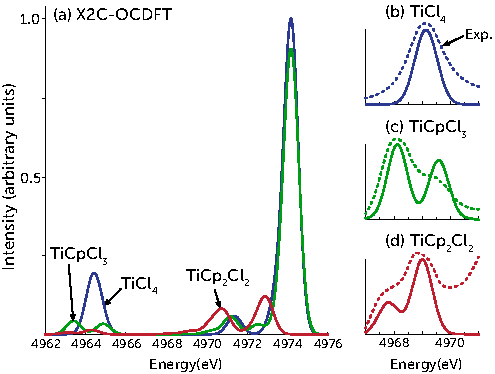
\includegraphics{figure_4.pdf}
	\caption{(a) Near-edge X-ray absorption spectrum of TiCl$_4$, TiCpCl$_3$, and TiCp$_2$Cl$_2$ computed with X2C-OCDFT at the B3LYP/un-cc-pVDZ level of theory.  (b)--(d) Comparison of the onset of the pre-edge experimental spectra (dotted line) with the X2C-OCDFT spectrum shifted by +4.7 eV to match the experimental pre-edge peak of TiCl$_4$ (solid line). Experimental curves taken from ref \citenum{TiCl4}. Ti K-edge for each molecule was simulated using 25 unique core-excited state (see supplementary material to see all excited states).}
	\label{fig:Ti-spectra}
\end{figure}

The unshifted X2C-OCDFT Ti K-edge peaks of TiCl$_4$, TiCpCl$_3$, and TiCp$_2$Cl$_2$ are reported in Table~\ref{table:pre-edge}, while Figure \ref{fig:Ti-spectra} shows a theoretical spectra simulated using 25 core excited states, together with a comparison of the shifted spectra with the experimental pre-edge features.\cite{TiCl4}
In accordance with experiment\cite{TiCl4}, X2C-OCDFT predicts the most intense absorption for TiCl$_4$ while the least intense for TiCp$_2$Cl$_2$. The relative ordering of the excitation energies of the three complexes predicated by OCDFT is in agreement with experiment as well. The most intense pre-edge feature for TiCl$_4$ occurs at 4964.4 eV (Expt. 4969.2 eV), while for TiCpCl$_3$, and TiCp$_2$Cl$_2$ it occurs at 4964.9 (Expt. 4968.1 eV) and 4964.3 (Expt. 4967.3) eV respectively.
It is also worth noting that the magnitude of the peak splitting is represented well by OCDFT. Our calculated pre-edge peaks for TiCpCl$_3$ and TiCp$_2$Cl$_2$ are split by 1.4 eV and 1.2 eV respectively, which are in excellent agreement with the experimental splitting of 1.4 eV observed for both compounds.

 \begin{table}[!b]
\caption{Transition energies (in eV) and relative oscillator strengths ($f$) for pre-edge transitions of TiCl$_4$, TiCpCl$_3$, and TiCp$_2$Cl$_2$ computed with X2C-OCDFT at the B3LYP/un-cc-pVDZ level of theory. Oscillator strengths shown are values relative to the most intense Ti K-edge transition of these three compounds (see supplementary material for detail).}
\begin{tabular}{ccccccc}
\toprule
State &   \multicolumn{2}{c}{\textbf{TiCl$_4$}}   & \multicolumn{2}{c}{\textbf{TiCpCl$_3$}} & \multicolumn{2}{c}{\textbf{TiCp$_2$Cl$_2$}} \\
& Energy & $f$ & Energy  & $f$ & Energy  & $f$ \\
     \cmidrule(r){2-3} \cmidrule(lr){4-5} \cmidrule(lr){6-7}  
1     &   4964.2 &             0.0945   & 4963.4 &    0.0202   & 4963.1 &                              0.0078 \\
2     &   4964.7 &             0.0940   & 4963.4 &    0.0191   &  4964.3 &                              0.0121 \\
3     &   4963.5 &             0.0002   & 4963.5 &    0.0164   & 4964.4 &                              0.0009 \\
4     &  4964.4  &             0.0947   &  4964.9 &   0.0220  & 4964.4 &                              0.0000 \\
5      & 4963.5         &      0.0000    & 4964.9 &   0.0217   & 4964.3 &                              0.0055 \\
\bottomrule
 	\end{tabular}
 	\label{table:pre-edge}
 \end{table}

The splitting of the pre-edge peak in the Cp-substituted compounds can be easily understood by examining the hole and particle orbitals that characterize each transition.
Figure \ref{fig:Ti-MOs} shows the particle orbitals for the five lowest excited states grouped according to which pre-edge feature they contribute.
In TiCl$_4$ all of the particle orbitals are combinations of Ti 3d, Ti 4p, and Cl 3p orbitals.
However, upon replacement of Cl with Cp ligands, the particle orbitals split into a group with no Cp ligand contribution (low energy) and a group with significant Cp ligand contribution (high energy).
Our assignment of the pre-edge peaks of TiCl$_4$ and TiCpCl$_3$ is in agreement with that of Ziegler et al.\cite{TiCl4-Zeigler}
However, our assignment of the Ti K-edge of TiCp$_2$Cl$_2$ is slightly different from the one reported by Ziegler\cite{TiCl4-Zeigler} and DeBeer.\cite{TiCl4}
Our OCDFT results suggest that the low energy peak is the result of a single transition while the second peak is a result of two transitions.
OCDFT predicts that these three peaks have similar intensities, which results in the 1:2 ratio of the absorption profile.
Ziegler et al.\cite{TiCl4-Zeigler} instead find that each peak in the K-edge of TiCp$_2$Cl$_2$ is due to a single transition, with the second transition being twice as intense as the first one.

\begin{figure*}[t!]
	\centering
	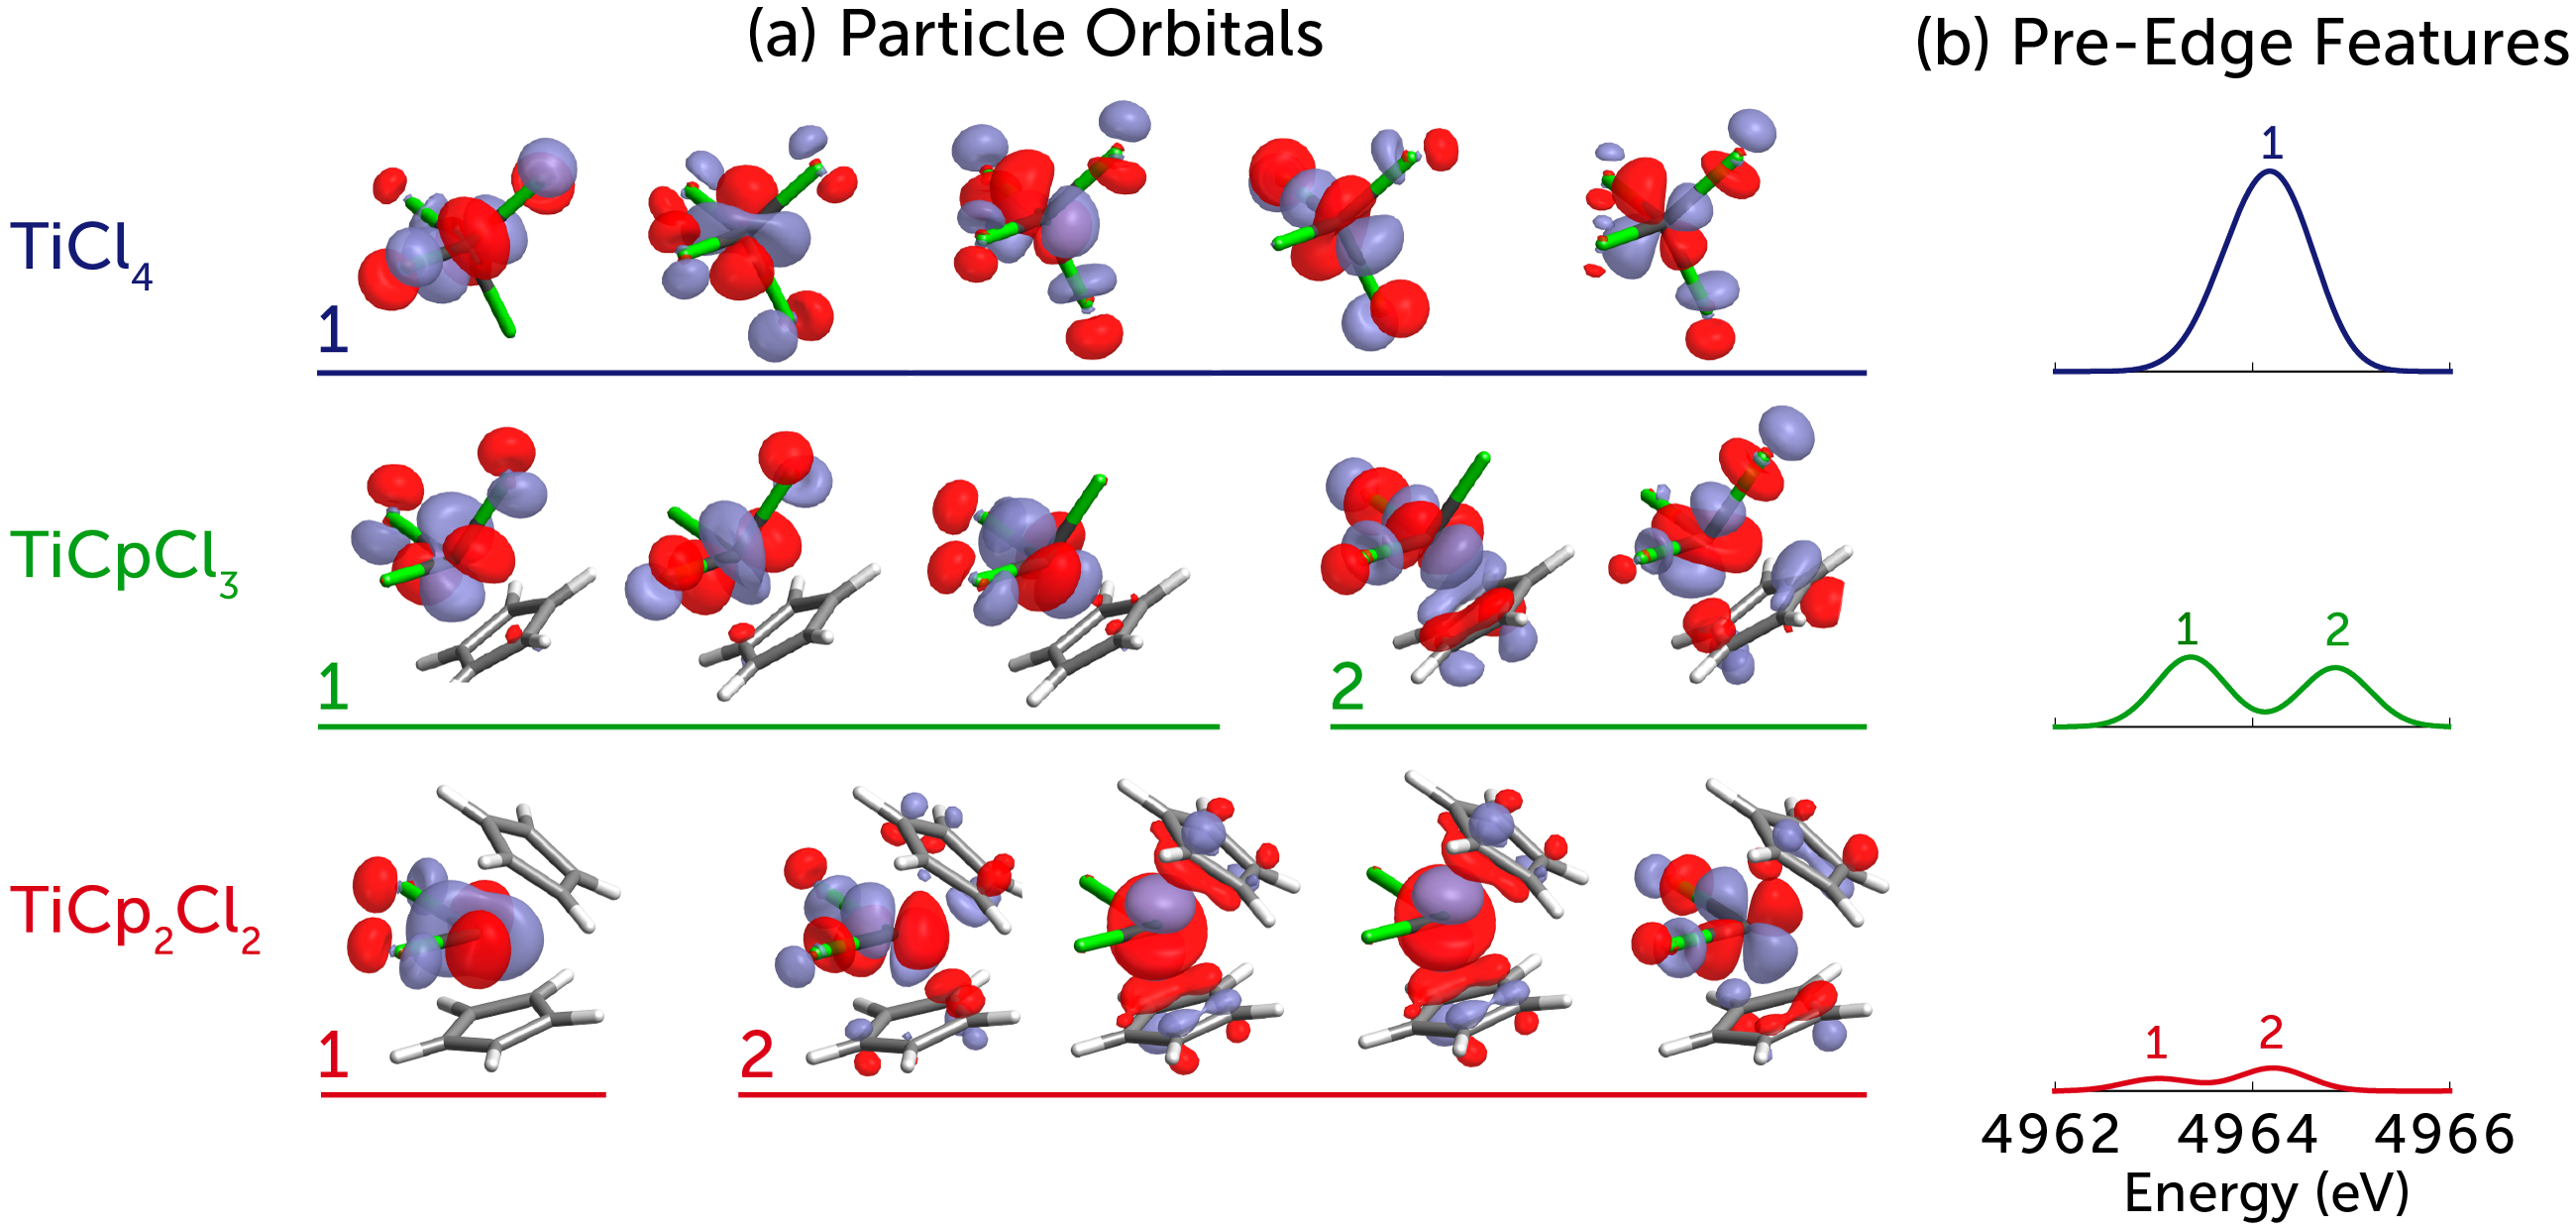
\includegraphics[width=6in]{figure_5.png}
	\caption{(a) Particle orbitals for the core excited states that contribute to the pre-edge features of TiCl$_4$, TiCpCl$_3$, and TiCp$_2$Cl$_2$ and (b) corresponding spectral features.}
	\label{fig:Ti-MOs}
\end{figure*}

To elucidate the nature of the Ti pre-edge features we generated natural atomic orbitals (NAOs),\cite{NBOs} for ground and excited states using the \textsc{janpa}\cite{nikolaienko_janpa:_2014} software interfaced with \textsc{psi4}\cite{PSI4}.
In Table \ref{table:4p_character} we compare the change in orbital shell occupation for each state that contributes to the pre-edge features of the NEXAS spectrum of TiCl$_4$, TiCpCl$_3$, and TiCp$_2$Cl$_2$.
Our analysis reveals that the pre-edge excitations consist mostly of transitions from Ti s to Ti d orbitals and are accompanied by a small increase in population of the Ti p orbitals, and (on average) a decrease in the population of the Cl p shell.

\begin{table*}[t!]
\footnotesize
	\caption{Change in the natural orbital population numbers of the Ti p, Ti d, Cl p shells computed for the Ti pre-edge excitations of TiCl$_4$, TiCpCl$_3$, TiCp$_2$Cl$_2$.}
	\begin{tabular}{lrrrrrrrrr}
		\toprule
		 &  \multicolumn{3}{c}{$\Delta$Ti$_\text{p}$}  & \multicolumn{3}{c}{$\Delta$Cl$_\text{p}$} &  \multicolumn{3}{c}{$\Delta$Ti$_\text{d}$}  \\ \cmidrule(lr){2-4} \cmidrule(lr){5-7} \cmidrule(lr){8-10}
		State & {\text{TiCl$_4$}}  & {\text{TiCpCl$_3$}} & {\text{TiCp$_2$Cl$_2$}}& {\text{TiCl$_4$}}  & {\text{TiCpCl$_3$}} & {\text{TiCp$_2$Cl$_2$}}& {\text{TiCl$_4$}}  & {\text{TiCpCl$_3$}} & {\text{TiCp$_2$Cl$_2$}} \\ \cmidrule(lr){2-4} \cmidrule(lr){5-7} \cmidrule(lr){8-10}
1	&	0.0107	&	0.0066	&	0.0097	&	-0.2184	&	-0.0597	&	0.0051	&	1.1348	&	1.1614	&	1.2586	\\
2	&	0.0126	&	0.0076	&	0.0069	&	-0.3080	&	-0.0513	&	-0.0253	&	1.2111	&	1.1339	&	1.1613	\\
3	&	0.0063	&	0.0088	&	0.0048	&	-0.1790	&	-0.0437	&	-0.0920	&	1.1272	&	1.1256	&	1.0685	\\
4	&	0.0107	&	0.0055	&	0.0050	&	-0.1448	&	-0.0702	&	-0.1038	&	1.0623	&	1.0368	&	1.0633	\\
5	&	0.0064	&	0.0061	&	0.0094	&	-0.0920	&	-0.0829	&	-0.0806	&	1.0403	&	1.0291	&	1.0853	\\
\bottomrule
	\end{tabular}
	\label{table:4p_character}
\end{table*}

DeBeer et al.\cite{TiCl4} have argued that since the Ti 1s to Ti 3d transition is electric dipole forbidden, the pre-edge states must gain intensity through mixing with metal $\text{4p}$ and ligand $\text{3p}$ orbitals.
We have tried to investigate this issue by conducting a Mulliken analysis of the OCDFT transition dipole moment.
In OCDFT, the transition dipole moment for the excitation $\Psi^{(0)} \rightarrow \Psi^{(n)}$ is approximated by the matrix element:
\begin{equation}
\boldsymbol\mu_{0n} = \bra[1]{\Phi^{(n)}}\hat{\mathbf{r}} \ket[1]{\Phi^{(0)}} = \sum_{\mu\nu} D^{0n}_{\mu\nu} \bra{\chi_\mu} \hat{\mathbf{r}} \ket{\chi_\nu}
\end{equation}
where $D^{0n}_{\mu\nu}$ is a transition density matrix and $\bra{\chi_\mu} \hat{\mathbf{r}} \ket{\chi_\nu}$ is the dipole integral in the atomic orbital basis ($\{\chi_\nu\}$).
To analyze each transition we decompose the transition dipole moment into partial atomic contributions.
The contribution to the transition dipole moment arising from the angular moment shell $l_\mathrm{A}$ of a donor atom A to the shell $l_\mathrm{B}$ on the acceptor atom B is expressed as the restricted sum:
\begin{equation}
\label{eq:contribution}
\boldsymbol\mu_{0n} (\mathrm{A}_{l_\mathrm{A}} \rightarrow \mathrm{B}_{l_\mathrm{B}}) = \sum_{\mu \in \mathrm{A}_{l_\mathrm{A}}}\sum_{\nu \in \mathrm{B}_{l_\mathrm{B}}} D^{0n}_{\mu\nu} \bra{\chi_\mu} \mathbf{r} \ket{\chi_\nu}
\end{equation}

Table~\ref{table:ti_analysis_dipole} reports the dominant partial atomic contributions to the transition dipole moment for the pre-edge transitions of TiCpCl$_3$.
For each state we report the three largest contributions to the transition dipole moment, summed over all atoms of the same type.
This analysis reveals that for all pre-edge transitions,the dominant contribution to the transition dipole moment is due to the Ti 4p orbitals.
For example, the transition dipole moment of state 1 can be written as a dominant contribution from Ti s $\rightarrow$ Ti p transitions of magnitude $|\boldsymbol\mu|$ = 41.8$\times 10^{-5}$  au, plus two smaller contributions from ligand-ligand and Ti s $\rightarrow$ Cl p transitions with absolute transition dipole moments of 6.6$\times 10^{-5}$ and 6.4$\times 10^{-5}$ au, respectively.
Other contributions arising from all other combinations of atomic orbitals contribute with a partial transition dipole moment equal to 7.3$\times 10^{-5}$ au.
Note that in many instances the three components of the partial dipole moment have different phases and approximately cancel out.
We observe this pattern also for other pre-edge transitions of TiCpCl$_3$ reported in table~\ref{table:ti_analysis_dipole} and for all transitions of TiCl$_4$ and TiCp$_2$Cl$_2$ (see the supplementary material for a full table of all significant atomic contributions to the pre-edge transitions of the three organotitanium complexes).
In order to assess the stability of this analysis with respect to the size of the basis set, we computed the N$_{1\text{s}}$ $\rightarrow \pi^*$ transition in HCN with six different basis sets: the cc-pV$X$Z series and the corresponding fully uncontracted basis sets, un-cc-pV$X$Z (with $X$ = D, T, Q). As expected, there is variation in the results, however, in all six cases, the most intense atomic contribution was classified as N$_{ \rm s}$ $\rightarrow$ N$_{\rm p}$.

Overall, our OCDFT analysis allows us to quantify the contribution of each atom and orbital shell to the NEXAS peak intensity.We found that peak intensity is acquired mainly from Ti 1s $\rightarrow$ Ti 4p excitations, a result that is in agreement with that proposed by DeBeer et al.\cite{TiCl4}
Interestingly, Ti 1s $\rightarrow$ Cl 3p excitations produce smaller contributions to the total peak intensity, despite the fact that on average the pre-edge transitions are accompanied by a larger change in the occupation of Cl p orbitals than Ti 4p orbital.
This is likely to result from smaller overlap of Ti 1s and Cl p orbitals, which implies a smaller transition dipole moment integral.

\begin{table*}[t!]
	\centering
	\caption{Partial atomic contributions to the transition dipole moment (in atomic units) computed for the pre-edge features of TiCpCl$_3$.}
	\begin{tabular}{lcccc}
		\toprule
		Contribution                  &     $\mu_x$ &     $\mu_y$ &     $\mu_z$ & $|\boldsymbol\mu|$ \\ \midrule
\multicolumn{5}{c}{{\bf{State 1}}}   \\
Ti$_{\rm s}$ $\rightarrow$ Ti$_{\rm p}$ & $-$0.000395 & $-$0.000079 & $-$0.000113 & 0.000418 \\
Cl$_{\rm p}$ $\rightarrow$ Cl$_{\rm p}$ & +0.000062 & +0.000012 & +0.000018 & 0.000066 \\
Ti$_{\rm s}$ $\rightarrow$ Cl$_{\rm p}$ & $-$0.000006 & +0.000003 & $-$0.000064 & 0.000064 \\
Other       & $-$0.000007 & +0.000002 & +0.000073 & 0.000073 \\
\multicolumn{5}{c}{{\bf{State 2}}}   \\
Ti$_{\rm s}$ $\rightarrow$ Ti$_{\rm p}$ & +0.000119 & $-$0.000321 & $-$0.000228 & 0.000411 \\
Ti$_{\rm s}$ $\rightarrow$ Cl$_{\rm p}$ & +0.000013 & $-$0.000000 & $-$0.000143 & 0.000144 \\
Ti$_{\rm s}$ $\rightarrow$ C$_{\rm p}$ & $-$0.000005 & $-$0.000019 & +0.000109 & 0.000111 \\
Other       & $-$0.000027 & +0.000061 & +0.000076 & 0.000101 \\
\multicolumn{5}{c}{{\bf{State 3}}}   \\
Ti$_{\rm s}$ $\rightarrow$ Ti$_{\rm p}$ & $-$0.000038 & $-$0.000289 & +0.000250 & 0.000384 \\
Ti$_{\rm s}$ $\rightarrow$ Cl$_{\rm p}$ & $-$0.000014 & $-$0.000020 & +0.000171 & 0.000173 \\
Ti$_{\rm s}$ $\rightarrow$ C$_{\rm p}$ & +0.000009 & $-$0.000000 & $-$0.000126 & 0.000126 \\
Other       & +0.000016 & +0.000057 & $-$0.000098 & 0.000114 \\
\multicolumn{5}{c}{{\bf{State 4}}}   \\
Ti$_{\rm s}$ $\rightarrow$ Ti$_{\rm p}$ & $-$0.000324 & $-$0.000299 & +0.000003 & 0.000441 \\
Cl$_{\rm p}$ $\rightarrow$ Cl$_{\rm p}$ & +0.000135 & +0.000128 & +0.000005 & 0.000186 \\
C$_{\rm p}$ $\rightarrow$ C$_{\rm p}$ & $-$0.000065 & $-$0.000061 & $-$0.000007 & 0.000089 \\
Other       & $-$0.000021 & $-$0.000015 & +0.000001 & 0.000026 \\
\multicolumn{5}{c}{{\bf{State 5}}}   \\
Ti$_{\rm s}$ $\rightarrow$ Ti$_{\rm p}$ & +0.000304 & $-$0.000313 & +0.000004 & 0.000436 \\
Cl$_{\rm p}$ $\rightarrow$ Cl$_{\rm p}$ & $-$0.000128 & +0.000134 & +0.000003 & 0.000185 \\
C$_{\rm p}$ $\rightarrow$ C$_{\rm p}$ & +0.000060 & $-$0.000062 & +0.000002 & 0.000086 \\
Other       & +0.000021 & $-$0.000024 & $-$0.000007 & 0.000033 \\
		 \bottomrule
	\end{tabular}
	\label{table:ti_analysis_dipole}
\end{table*}

\section{Discussion and Conclusions}

In this study we have combined orthogonality constrained DFT (OCDFT) with the spin-free exact two-component relativistic (X2C) Hamiltonian, and used this as a tool to analyze scalar relativistic effects in the context of core electron excitations.  When relativistic effects are not significant, OCDFT consistently reproduces experimental core-valence excitation energies within 1 eV.
The influence of scalar relativistic effects can already be seen in the failure of nonrelativistic OCDFT at computing core excitation energies of transitions involving the 1s orbital of second-row elements. 
For example, the magnitude of relativistic effects for the Si $\text{1s}$ $\rightarrow$ $\sigma^*$ excitation in SiH$_4$ is estimated to be 4.3 eV, but for the Cl $\text{1s}$ $\rightarrow$ $\sigma^*$ excitation in HCl this figure increases to 10.1 eV. 
We demonstrated that by combining OCDFT with a scalar relativistic Hamiltonian and the B3LYP functional, core excitation energies for second row elements can be computed with an average error of 2.3 eV (from a test set of 10 transitions), a substantial improvement over the 10.3 eV average error observed with the nonrelativistic OCDFT.

Using a class of well studied organotitanium compounds (TiCp$_{n}$Cl$_{4-n}$, n = 2--4), we have demonstrated the utility of the X2C-OCDFT method as a tool to compute accurate transition metal K-edge spectra.
The inclusion of scalar relativistic effects is mandatory to obtain near-quantitative agreement with experimental excitation energies.
For example, for TiCpCl$_3$ we find that a non-relativistic OCDFT treatment predicts excitation energies with an error of about 35 eV.
Once augmented with X2C, the OCDFT error is reduced to 4.8 eV, which is a marked improvement results from relativistic TDDFT (18 eV)\cite{TiCl4-Zeigler}. 
We find that X2C-OCDFT consistently underestimates the pre-edge features of Ti 1s transitions by ca. 5 eV, which is commensurate with our analysis of second row 1$\text{s}$ excitations (MAE = 2.3 eV, max error = 3.6 eV).
In other words, the relative error of X2C-OCDFT Ti K-edge excitation energies is of the order of 0.1\%.
A large portion of the remaining error is most likely due to the use of an approximate functional for the excited state employed in the theory (adiabatic approximation), but also the increased importance of non-scalar relativistic effects (spin-orbit coupling, finite nuclei effects, etc.) that are not captured by spin-free scalar relativistic Hamiltonians.

To gain insight into the nature of the Ti K-edge excitations, we characterize the change in natural atomic orbital population and examine partial atomic contributions to the transition dipole moment of all states that contribute to the pre-edge features.
The character of the pre-edge transitions of the three organotitanium compounds as predicted by OCDFT is consistent with previous analyses,\cite{TiCl4,TiCl4-Zeigler}
however, in this study we developed an approach to quantify partial atomic contributions to the transition dipole moments.
This tool enables us to attribute most of the pre-edge peak intensity to excitations involving Ti 4p orbitals.  Ligand orbitals are found to give small contributions to the peak intensity.

What contributes to the improved performance of OCDFT with respect to TDDFT for core excitation energies?
Our evidence suggests that like other $\Delta$SCF based approaches,\cite{STEX,Besley-EOM-MOM,Thomas,Voorhis,Ziegler-1,Besley-Gill} OCDFT derives an advantage from the fact that it can properly describe charge-transfer excitations.\cite{Casida-TDDFT-CT-problem,Zeigler-TDDFT-CT-problem}
To illustrate this point, we computed the C and O K-edge spectrum of CO using various functionals and interpreted our data using a toy model of that captures the charge-transfer character of core excitations.
Our analysis suggests that a large source of the error in TDDFT arises from double counting the change in Coulomb energy that results from unpairing a core electron.
In the case of OCDFT, the effects of double counting the Coulomb repulsion is smaller, and the energy expression involves only local self-interaction terms.
We also note a stronger dependence of the TDDFT spectrum on the amount of Hartree--Fock exchange included in the functional.
Although shifted TDDFT will be comparable to OCDFT results, they are not identical, and there exists significant merit in performing OCDFT calculations since it yields more consistent predictions.
%In our analysis we have focused on the charge-transfer-like nature of core excited states.

One future application of this work is to extend OCDFT to the computation of L-edge spectra. The L-edge is composed of excitations from core 2p orbitals and simulation of the full spectrum will require proper treatment of spin-orbit coupling effects due to mixing of excitations from degenerate 2p orbitals. We would also like to explore the idea of using this orthogonality constrained excited state framework to build wave function based methods with the same advantages seen in OCDFT. This would allow us to create systematically improvable schemes that do not rely on approximate exchange-correlation functionals.


\section*{Acknowledgments}
This work was supported by start-up funds provided by Emory University. We would like to thank Dr. Lan Cheng for providing data to benchmark our implementation of X2C We would also like to acknowledge Dr. Tymofii Y. Nikolaienko for providing help with the JANPA software package. W.D.D. is supported by the National Science Foundation Graduate Research Fellowship under Grant No. 0000048655. Any opinion, findings, and conclusions or recommendations expressed in this material are those of the authors and do not necessarily reflect the views of the National Science Foundation.

{\footnotesize
\bibliography{biblio}
\bibliographystyle{achemso}
}
\end{document}